\documentclass[../main.tex]{subfiles}

\begin{document}
    % Hier soll eine Übersicht ("Big Picture") über die Struktur der Software bzw. des Systems gegeben werden.
    % Traditionelle Architekturansätze sprechen von "konzeptioneller Ansicht" oder "logischer Struktur", was oft zu Verwirrungen führt,
    % z.B.ob auch Implementationsdetails wie die verwende-ten Technologien enthalten sein sollen oder nicht
    % Für eine sinnvolle Gliederung in verschiedene Ebenen empfehlen wir den C4 Ansatz:
    %   •Context/System-Diagramm
    %   Ein Übersichtsdiagramm, welches das System und seine Abhängigkeiten und Aktoren zeigt.
    %
    %   •Container-Diagramm
    %   Zeigt eine Übersicht der verwendeten Technologien. Ein Container repräsentiert eine Lauf-zeitumgebung (z.B. Java App-Server, .NET, Ruby-Prozess, ...)
    %   in dem ein Teil ihres Programmes läuft oder einen Datenspeicher (Datenbank, Filesystem,....).
    %   Für die Kommunikation zwischen Containern wird normalerweise ein definiertes API verwendet (z.B. REST, RMI, JDBC, Messaging-Service, ...)
    %
    %   •Component-Diagramm
    %   Für jeden Container kann ein Komponenten-Diagramm gezeichnet werden, in welchem die Schlüsselkomponenten und ihre Beziehung untereinander dargestellt sind.
    %   Componenten definieren logische Kombination von Klassen, die zusammen eine bestimmte logische Funktionalität anbieten (z.B. Logging, Security, ...).
    %   Die Schnittstelle zwischen Componentenist typischerweise ein Interface (Interface-Klasse).
    %
    %   •Class-Diagramm (Klassendiagramm) -optional
    %   Dies ist die tiefste Ebene, in welcher das Zusammenspiel von Klassen innerhalb einer Componente visualisiert wird.
    %   Dies ist eine optionale Ebene, die nur verwendet wird um ganz spezifische Spezialitäten zu dokumentieren.
    %
    % Die ausführliche Idee und Beschreibung finden sie im Referenzbuch "Software-Architecture for Developers" [Simon Brown, Leanpub, 2015],
    % Kapitel "C4: context, containers, components and classes". Dieser Ansatz stellt sicher, dass jeweils nur Elemente auf der konzeptionell
    % gleichen Ebene mit-einander interagieren, sowie eine klare Trennung der Verantwortlichkeit und die Verwendung definierte Schnittstellen sichergestellt werden.
    % Zudem kann man zwischen den verschiedenen Ebenen wechseln um entweder mehr Details oder eine bessere Übersicht zu erhalten.
    % Die Diagramme sollten durch eine kurze Erläuterung des gezeigten und einer kurzen Zusam-menfassung für jeden Container/Componenten ergänzt werden.
    % In diesem Kapitel soll die Architektur so zusammengefasst werden, dass folgende Fragen be-antwortet werden:
    %   •Wie sieht die Übersicht (10km Vogelperspektive) aus?
    %   •Ist die Struktur klar?
    %   •Zeigt sie die wesentlichen Container und Technologien?
    %   •Zeigt sie die wesentlichen Komponenten und deren Interaktion?
    %   •Was sind die Schlüsselschnittstellen (API)? Nach aussen und zwischen den Komponenten.
    %
    %Dieses Kapitel muss in jedem Software-Guidebook enthalten sein.
	\section{Architektur}
	\subsection{Verwendete Technologien}
	\par Zur Entwicklung von \gls{hexxle} wird die Engine \gls{unity} verwendet. Als Programmiersprache wird \gls{csharp} verwendet. Neben der Entwicklung werden auch diverse Tools für das Projektmanagement verwendet. Im Folgenden eine kurze Übersicht über verwendete Technologien:

	\subsubsection{Funktionale Technologien}
	\begin{itemize}
		\item \gls{csharp}
		\item Unity-Version 2019.4.X LTS (long time support)
		\item Visual Studio bzw. Visual Studio Code
		\item Blender
	\end{itemize}
	\subsubsection{Administrative Tools}
	\begin{itemize}
		\item \href{https://github.com/hexxler/hexxle_game}{GitHub (Hexxle)}
		\item \href{https://github.com/hexxler/documentation}{GitHub (Dokumentation)}
		\item \href{https://hexxle.atlassian.net/jira/software/projects/HEXXLE/boards/1}{Jira}
		\item Whatsapp
		\item Microsoft Teams
		\item Parabol (Sprintretrospektiven)
	\end{itemize}

	\subsection{Big Picture CHANGE NAME}
	\par Das Entwicklerteam benutzt Unity, Visual Studio und Blender für die Entwicklung von \gls{hexxle}. Unity agiert hier als zentraler Ankerpunkt des Projekts und ist für die Vernetzung aller relevanten Systeme zuständig. Für die Versionierung wird GitHub verwendet. Das Projektmanagement findet mithilfe von Jira statt.
	\begin{figure}[H]
	\centering
	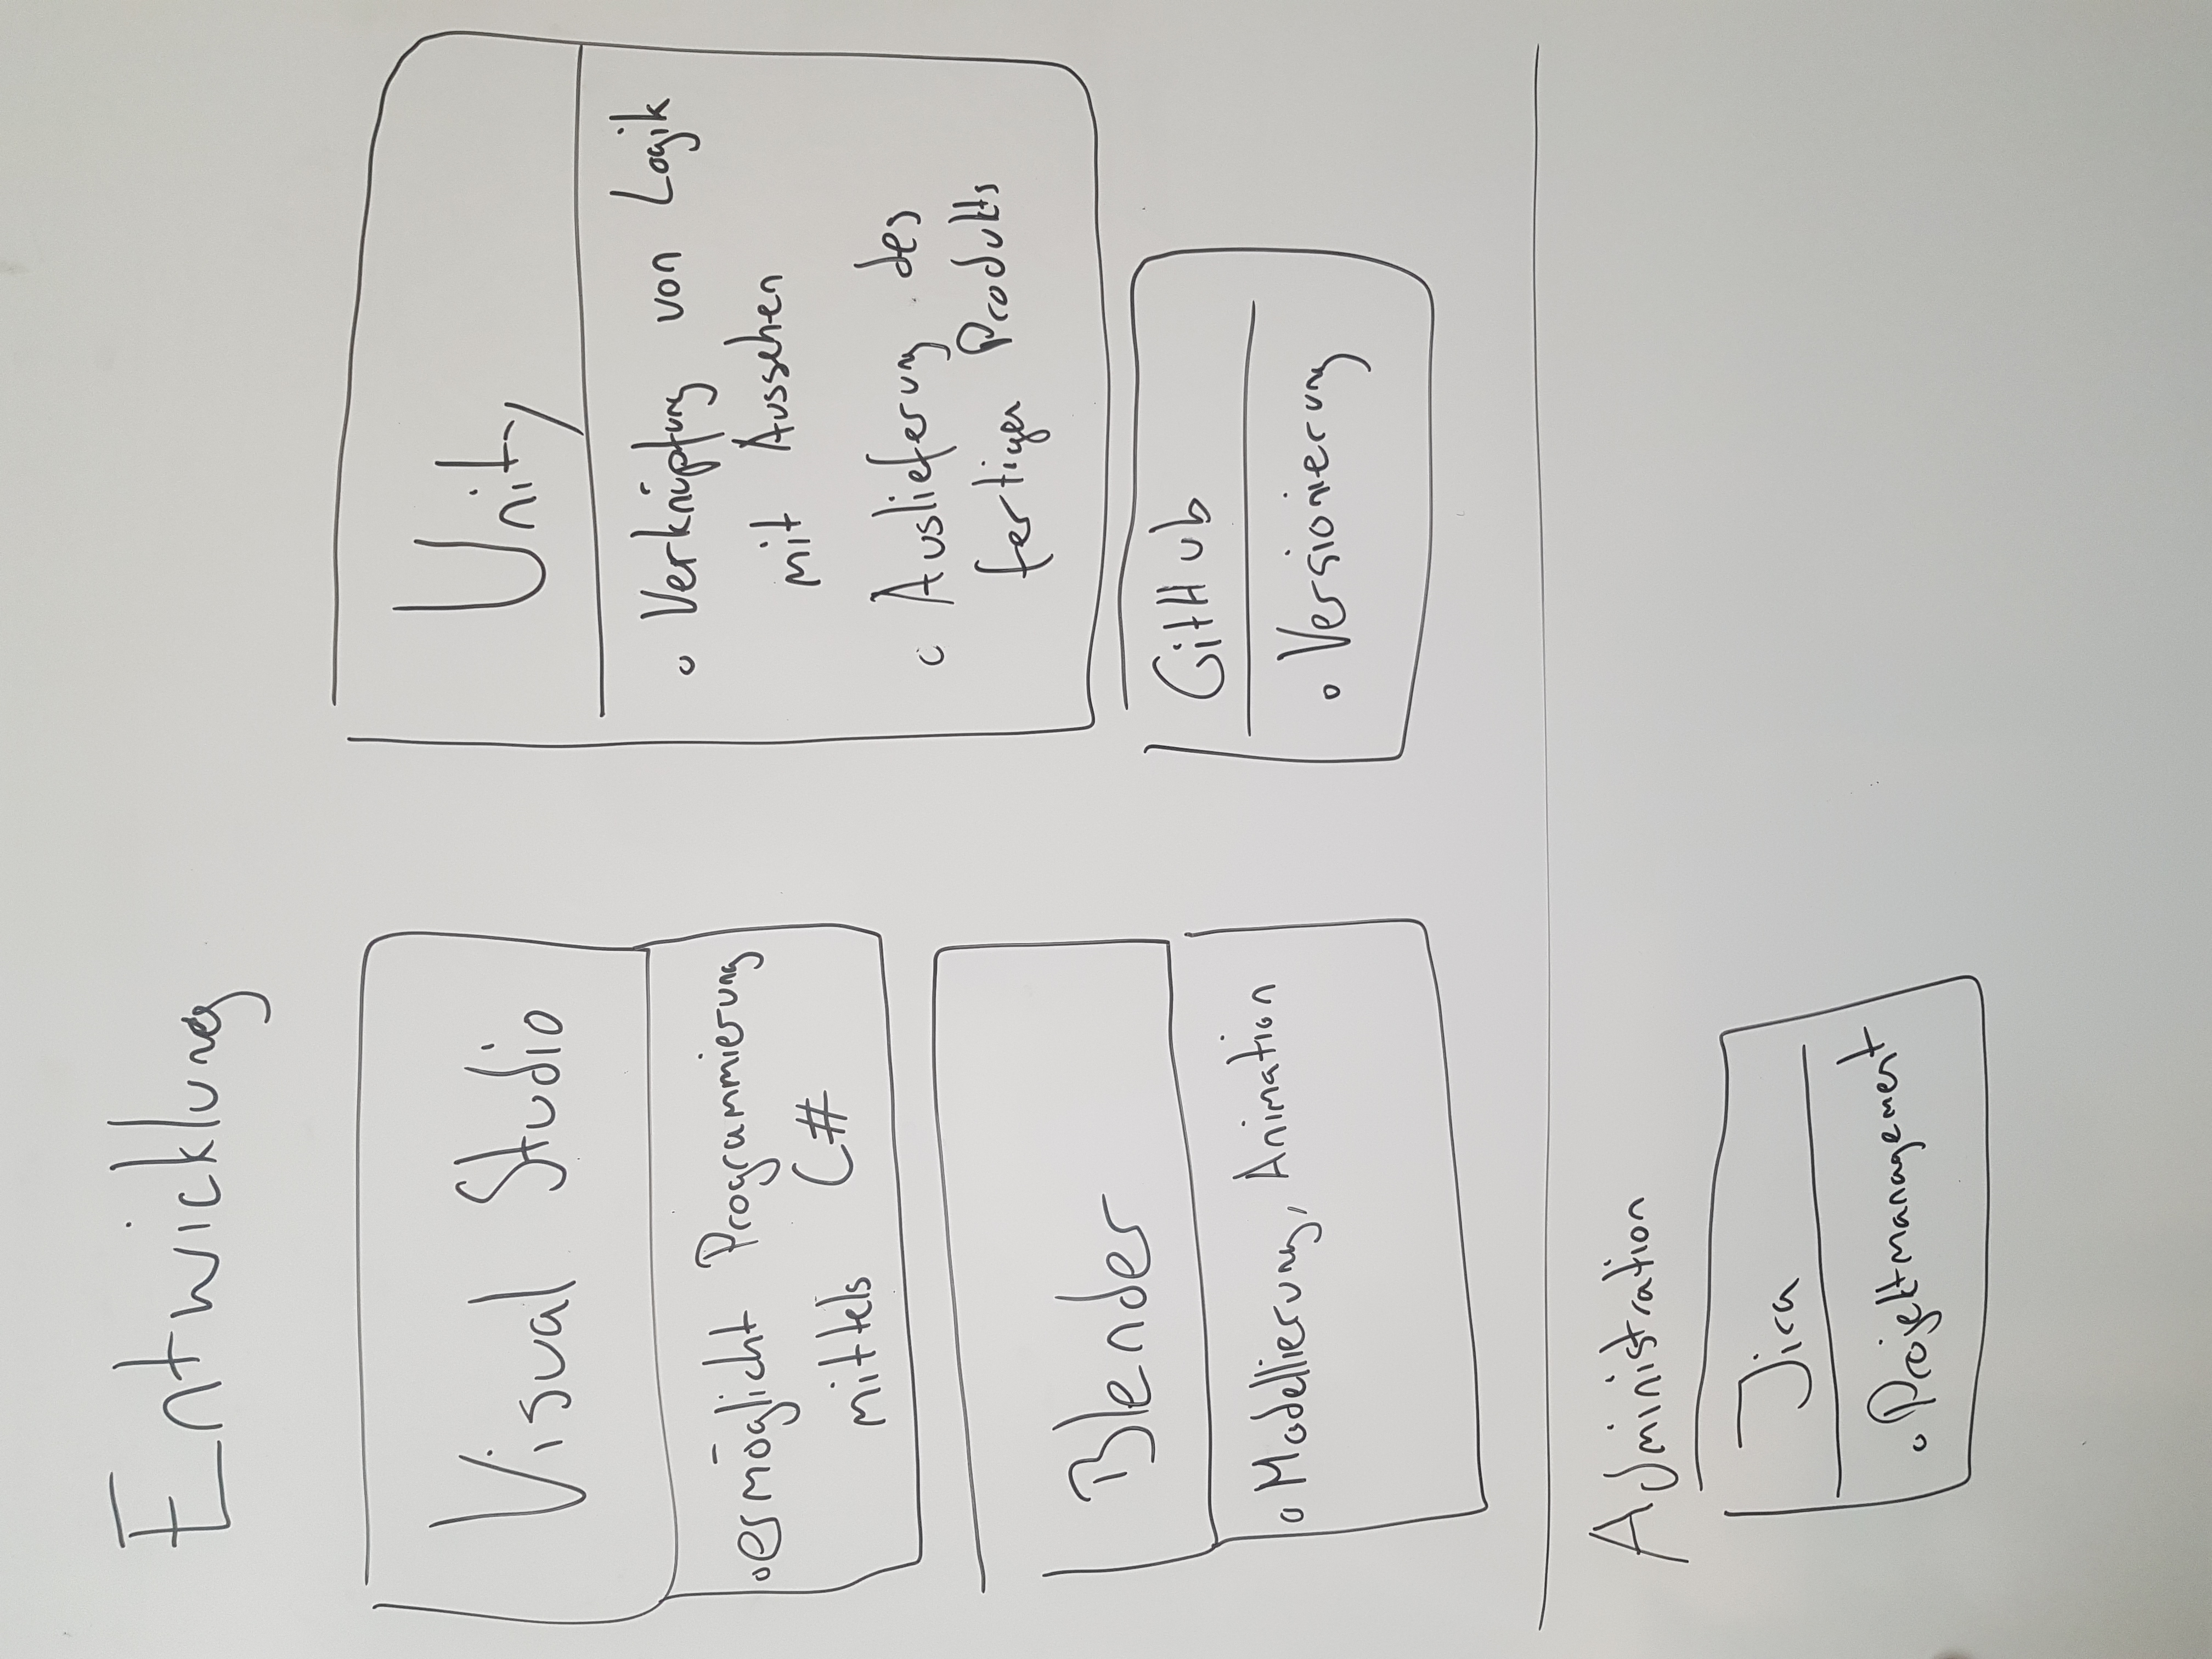
\includegraphics[angle=-90, width=0.6\linewidth]{big_picture.jpg}
	\end{figure}

	\subsection{Unity/Code-Architektur}
	\label{section:UnityCodeArchitektur}
	\par Unity strukturiert den Aufbau einzelner Bereiche des Spiels mittels Szenen. Szenen wiederum beinhalten eine variable Anzahl GameObjects, welche wiederum aus diversen Komponenten und eventuell weiteren GameObjects bestehen. MonoBehaviours können den GameObjects als Komponente hinzugefügt werden und enthalten mit dem GameObject assoziierten Code. MonoBehaviours verwenden Interfaces, um mit der eigentlichen, Unity agnostischen Logik des Spiels zu interagieren.
	\par Die Spiellogik wird in regulären C\#-Klassen implementiert und spiegelt die Spielregeln wieder, ohne etwas über die schlussendliche Darstellung wissen zu müssen. Klassen der Spiellogik verwenden wenn möglich keine Funktionen der UnityEngine. Eine Ausnahme stellen hier beispielsweise Structs wie Vector2 und Vector3 dar. Klassen der Spiellogik implementieren Interfaces und machen somit klar definierte Funktionalitäten nach aussen zugänglich.
	\par Die Spiellogik verwendet Datenklassen und Structs, die kein konkretes Verhalten der Spielregeln implementieren, sondern lediglich Zustände speichern.
	\begin{figure}[H]
		\centering
		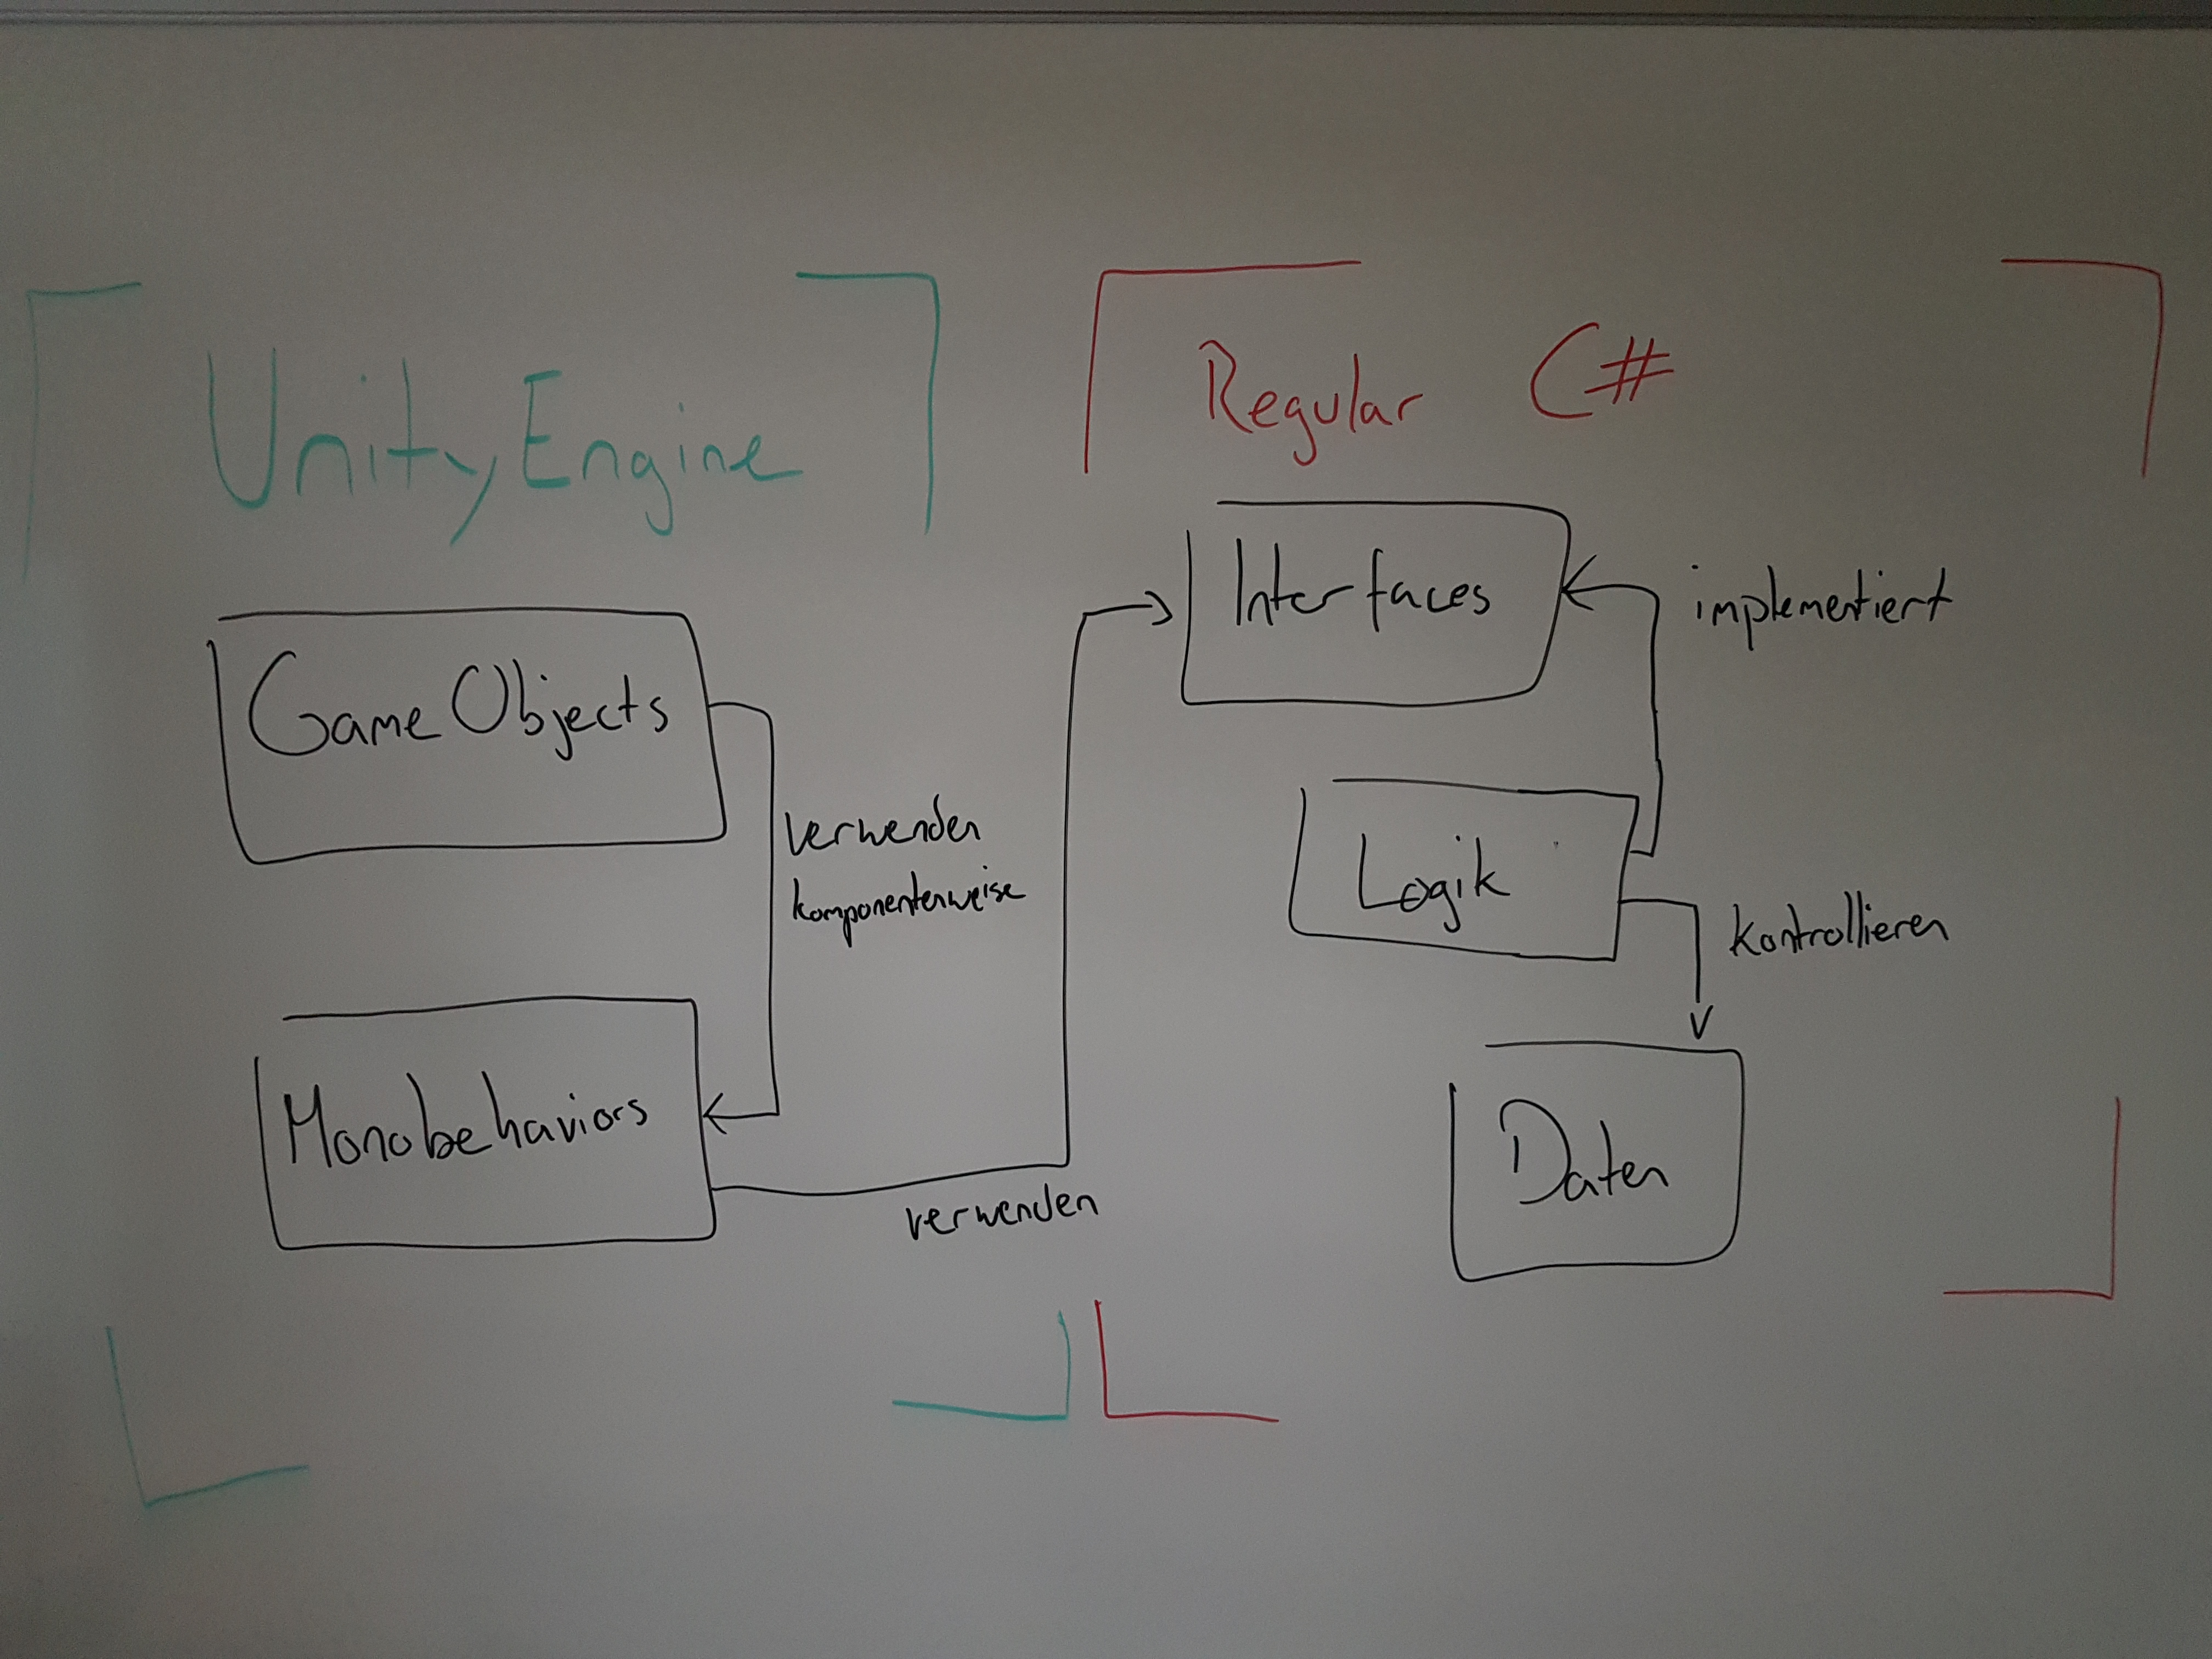
\includegraphics[angle=0, width=0.6\linewidth]{Container_View.jpg}
	\end{figure}
	
	\subsection{MonoBehaviours-Architektur}
	\par Die verschiedenen MonoBehaviours interagieren einerseits mit Komponenten der Unity GameObjects (MeshRenderer, Transform, UI-Elemente etc.) und andererseits mit Interfaces aus der regulären C\#-Umgebung.
	\todo{Bild über MonoBehaviour Architektur}
	\subsection{C\#-Code-Architektur}
	\todo{Text über C\# Code Architektur}
	\todo{Bild über C\# Code Architektur}
\end{document}